			From \eqref{eq:line-rank-2},
the collinearity matrix can be expressed as
 \begin{align}
			    \myvec{-5 & -2
			    \\
			    5 & 2 }  
			    \xleftrightarrow[]{R_2 \leftarrow {R_1 + R_2}}
			    \myvec{	    -5 & -2  
			    \\
			    0 & 0}  
\end{align}
which is a rank 1 matrix.  See 
		\figref{fig:11/10/2/20}.
	\begin{figure}[!ht]
		\centering
 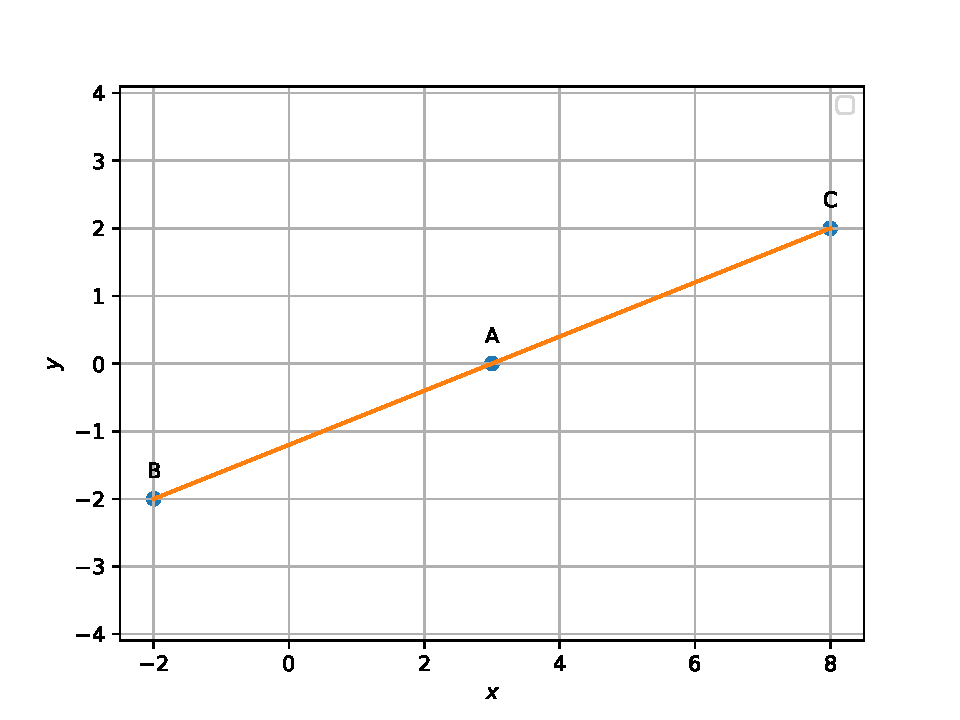
\includegraphics[width=\columnwidth]{chapters/11/10/2/20/figs/figs6.pdf}
		\caption{}
		\label{fig:11/10/2/20}
  	\end{figure}
